\section{Cele i~problematyka pracy}

\subsection{Cele}

\subsubsection{Przybliżenie metodologii Scrum}

Jednym z~podstawowych celów pracy inżynierskiej jest przedstawienie (prezentacja) wykorzystanych w~niej technologii, narzędzi, metod itp. Ze~względu na~użycie podczas pisania mojej pracy metodologii Scrum \cite{scrumalliance} (używanej powszechnie w~małych i~średnich firmach -- nie tylko programistycznych) zamierzam opisać tę~metodologię i~zaprezentować w~prosty sposób jej przebieg.

\subsubsection{Przybliżenie (popularyzacja) technologii Ruby~on~Rails} \label{cele.ror}

Ruby~on~Rails (często nazywany RoR lub po~prostu Rails) to~framework open source do~szybkiego tworzenia aplikacji webowych stworzony głównie przez duńskiego programistę Davida Heinemeiera Hanssona w~ramach pracy nad oprogramowaniem Basecamp\footnote{Patrz: \url{http://basecamphq.com/}}. Rails to~w~pełni wyposażone środowisko do~tworzenia aplikacji internetowych opartych o~bazy danych zgodnie ze~wzorcem MVC (Model-View-Controller). Ruby~on~Rails daje programiście środowisko w~pełni oparte o~język programowania Ruby -- od~Ajax'a dostępnego w~widokach (View), do~zapytania i~odpowiedzi w~kontrolerach i~logice biznesowej modeli.


Tuż po~pojawieniu się Ruby~on~Rails na~forum publicznym okrzyknięto go~sensacyjnym. Tim O'Reilly, Założyciel O'Reilly Media mówił\footnote{Źródło: \url{http://www.rubyonrails.pl/cytaty}} ,,Ruby on Rails jest przełomem w~dziedzinie programowania aplikacji internetowych. Potężne aplikacje, których tworzenie do~tej pory zabierało tygodnie czy miesiące, są~teraz tworzone dosłownie w~kilka dni.''


Niestety -- w~ciągu ostatnich trzech lat spadło zainteresowanie technologią Ruby~on~Rails (patrz wykres \ref{fig.wykres.googleresearch}). Programiści coraz rzadziej sięgają po~ten produkt wybierając nowsze rozwiązania takie jak Django\footnote{Patrz: \url{http://www.djangoproject.com/}} napisane w~języku Python\footnote{Patrz: \url{www.python.org}}. Nadzieją na~poprawienie tej sytuacji jest nowo wydana -- trzecia wersja frameworku Ruby~on~Rails oraz~ciągły rozwój dodatków -- wtyczek \texttt{gem}. Dlatego też chcę przybliżyć tę~technologię i~zachęcić do~jej używania.

\begin{figure}[!t]
\centering
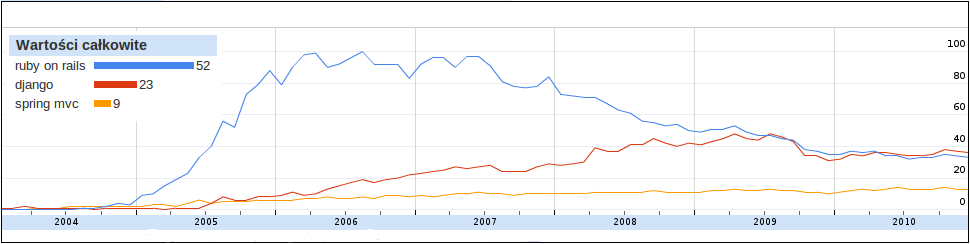
\includegraphics[width=\textwidth]{obrazki/googleresearch.png}
\caption{Statystyka wyszukiwarki Google na~temat znanych aplikacji szkieletowych (źródło: \url{http://www.google.com/insights/search/\#cat=5\&q=Ruby\%20on\%20Rails\%2CDjango\%2CSpring\%20MVC\&cmpt=q}).}
\label{fig.wykres.googleresearch}
\end{figure}

Liczby na~wykresie \ref{fig.wykres.googleresearch} wskazują, ile wyszukiwań przeprowadzono na~podstawie określonego hasła w~porównaniu do~łącznej liczby wyszukiwań przeprowadzonych w~Google w~tym czasie. Wartości te~nie odzwierciedlają bezwzględnej liczby wyszukiwań, ponieważ dane są~znormalizowane i~przedstawione na~skali od~0 do~100. Każdy punkt na~wykresie jest dzielony przez wartość najwyższego punktu. Jeśli ilość danych jest za~mała, podawana jest wartość 0. Liczby wyświetlane nad wykresem obok wyszukiwanych haseł stanowią podsumowania lub wartości łączne\footnote{Źródło: \url{http://www.google.com/support/insights//bin/answer.py?hl=pl\&answer=87285}}.

\subsubsection{Opis zastosowania technologii Ruby~on~Rails w~problemie stworzenia systemu aukcyjnego}

Technologia Ruby~on~Rails umożliwia proste tworzenie aplikacji webowych dowolnego typu. Dla zaprezentowania jej możliwości wybrałem system aukcyjny jako przykład aplikacji webowej stworzonej w~tym środowisku. Wybór ten nie jest przypadkowy -- do~tej pory nie znalazłem przykładowego systemu aukcyjnego napisanego przy użyciu aplikacji szkieletowej Ruby~on~Rails\footnote{Jedynym możliwym gotowym rozwiązaniem dla wykorzystania aplikacji webowej w~celu wystawiania aukcji/prowadzenia licytacji jest zastosowanie wtyczki % TODO nazwa i url
dla systemu CMS % TODO nazwa i url CMS - chyba spree
napisanego w~Ruby~on~Rails.}.


Pomysł jednak nie jest nowatorski -- w~sieci oraz~w~wielu pozycjach książkowych znajdują się przykłady wykonania sklepów internetowych, które są~w~budowie bardzo podobne do~systemów aukcyjnych.


System aukcyjny to~niezwykle rozwlekły i~obszerny temat. Projekt tego typu zatem może być bardzo rozbudowany. Właśnie z~tego względu zakładam, że~mój projekt nie będzie ,,dokończony''. Celem nie jest tu~wykonanie całego projektu ,,od~początku do~końca'' a~jedynie prezentacja możliwości jakie oferuje Ruby~on~Rails.

\subsubsection{Przedstawienie prototypu systemu aukcyjnego}

Wraz ze~stworzeniem prototypu systemu aukcyjnego prezentuję podstawowe rozwią\-zania dla tego rodzaju problemu. Zagadnienie stworzenia systemu aukcyjnego jest problemem typowym dla dziedziny inżynierii oprogramowania. Wymaga wybrania i~opracowania rozwiązań technicznych i~technologicznych oraz~określenia metodyki pracy nad danym zagadnieniem.


Stworzony przeze mnie prototyp jest swego rodzaju prezentacją zastosowanych w~nim technologii oraz~przykładowych rozwiązań.

\subsubsection{Ocena możliwości wdrożenia proponowanych rozwiązań}

Do~pełnego przedstawienia cyklu pracy nad projektem wykonanym w~technologii Ruby~on~Rails potrzebne jest przedstawienie metod wdrożenia aplikacji webowej oraz~zaproponowanie sposobu jej konserwacji. W~tym celu mam zamiar przybliżyć jedne z~najprostszych znanych mi sposobów wdrożenia aplikacji Ruby~on~Rails.
